\documentclass{article}
\usepackage[utf8]{inputenc}
\usepackage{graphicx}
\usepackage{listings}


%Import the natbib package and sets a bibliography  and citation styles
\usepackage{natbib}
\bibliographystyle{abbrvnat}



\title{Jaguares de Sudamerica}
\author{Angel Luis Robles Fernandez}
\date{September 2020}

\begin{document}

\maketitle

\section{Resumen}
A continuación se presentan estadísticos sumarios y representaciones gráficas análisis sobre poblaciones de jaguares en Sudamérica



\section{Metodología}

Se leyó el archivo vfc producido por stacks a través de la herramienta vcfR
(\citealt{knaus2017}). También se revisó que todas las muestras en el VCF estubieran en la lista de datos de población del archivo \textbf{pop\_mat\_25smp.txt}

Con la misma herramienta vcfR se convirtió la lectura en un objeto de clase genlight para ser manipulado posteriormente por el paquete adegenet (\citealt{jombart2011}). Este formato permite guardar genotipos de SNPs binarios de manera compacta. El genlight puede ser utilizado en cualquier nivel de ploidía. En este caso se ajustó a un nivel de diploidía (2 conjuntos de cromosomas). Además se asignó cada población a cada muestra en el objeto de genlight. 
Se utilizó el paquete poppr (\citealt{kamvar2015novel}) para obtener una matriz de distancias bit a bit, esto es una matriz de disimilitud entre las muestras, comparando cuánta información comparte una muestra con respecto a otra. \ref{fig:heatmap}

Posteriormente se generó un árbol genético entre estas distancias con el mismo paquete poppr y la función aboot. Esta función calcula un dendograma utilizando la distancia entre genotipos individuales. El mismo paquete permite construir la red recubridora mínima (minimum spanning network) entre las muestras. Esta red es una transformación del dendograma (árbol) que es un grafo en otro grafo que mantiene conectadas todas las muestras. Cada nodo en el grafo representa un genotipo multilocus. Las aristas en el grafo representan las  distancias genéticas que conectan los genotipos multilocus. \ref{fig:tree1} 

Los análisis de componentes principales  se han utilziado por décadas para extraer varios tipos de información de datos genéticos. La principal fortaleza de PCA es su capacidad para identificar estructuras genéticas en conjuntos de datos muy grandes dentro de un tiempo computacional insignificante y la ausencia de cualquier suposición sobre el modelo genético de población subyacente (\citealt{jombart2008adegenet}). Sin embargo, el PCA carece de características esenciales para investigar la estructura genética de poblaciones biológicas. En primer lugar no proporciona una evaluación de pertenencia a un grupo, y requeriría una definición \textit{a priori} de los clusters para estudiar la estructura de la poblaci
ón. Para evaluar las relaciones entre los diferentes clusters, un método adecuado debe centrarse en la variabilidad entre grupos, sin tener en cuenta la variación dentro del grupo. Por esta razón se utilizaó el método de análisis discriminante de componentes principales. Este método está diseñado para identificar y describir clusters de individuos relacionados genéticamente. Cuando se tiene una carencia de priors por grupo, DAPC utiliza el algoritmo k-medias de manera secuencial para inferir cluster genéticos. Este enfoque permite extraer información de los datos genéticos proporcionando una asignación de los individuos a algún grupo en particular.  \ref{fig:PCA_DA} 

Se hicieron ambos análiis, tanto PCA, como DA, se obtuvo la varianza explicada para cada valor propio del PCA, así como la gráfica del espacio PCA para las poblaciones. Sin embargo se pudo asignar a cada muestra una población utilizando el análisis discriminante.\ref{fig:estructura} 



\section{Resultados}

A continuación se presentan los resultados explicados en la metodología anterior. 
Se puede observar del boxplot que hay mjuestras que tienen mucha varianza de su distancia con respecto a las demás muestras. Además del mapa de calor se observa que existen algunos grupos (clusters) de muestras sin conocer la estructura de las poblaciones. Con esta inferencia se construyó un dendograma y se transformó en un grafo de expansión mínima donde se observan dos grandes grupos de genotipos. 
\begin{figure}[h]
    \centering
    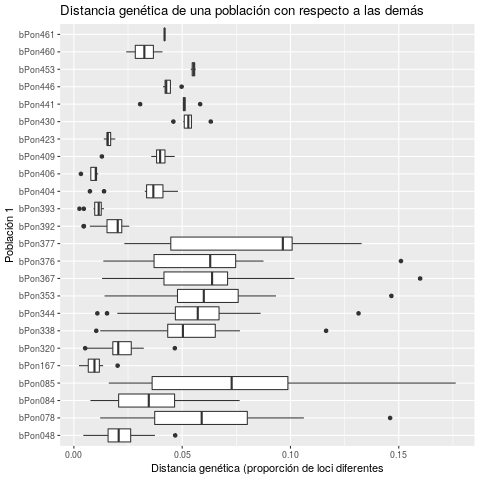
\includegraphics[width=0.4\textwidth]{boxplot_distancia.png}
    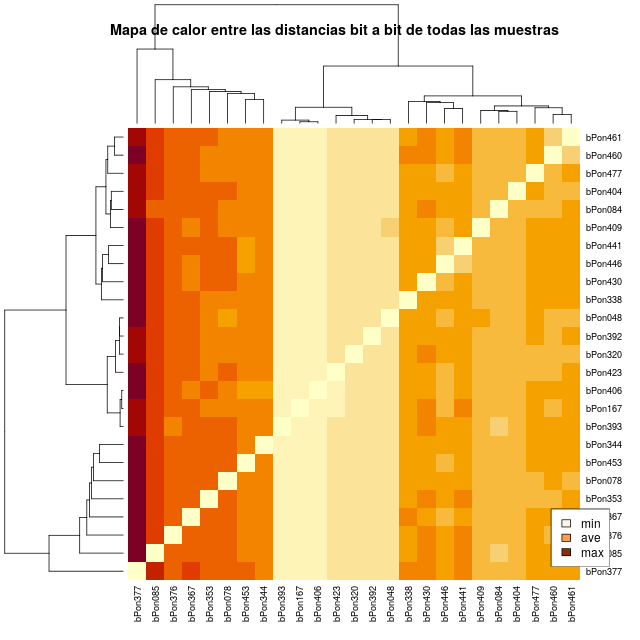
\includegraphics[width=0.4\textwidth]{heatmap_distance.png}
    \caption{Distancia media entre una población con respecto a las demás. A la derecha, mapa de calor entre las muestras}
    \label{fig:heatmap}
\end{figure}


\begin{figure}[h]
    \centering
    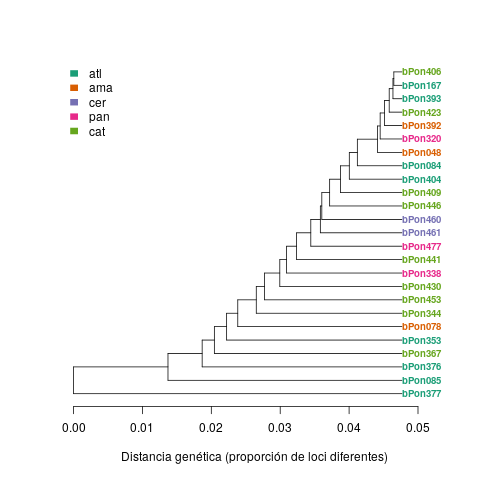
\includegraphics[width=0.45\textwidth]{arbol_jaguar.png}
    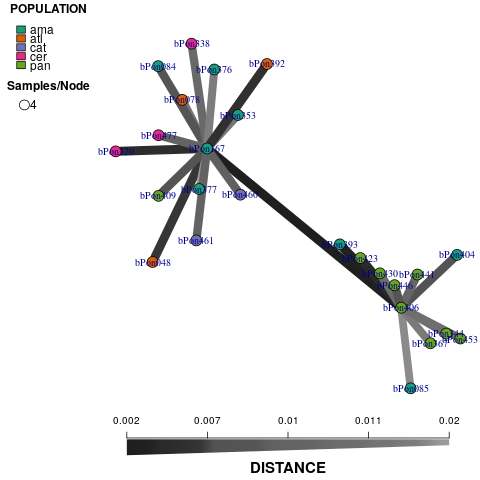
\includegraphics[width=0.45\textwidth]{grafo_red_jaguar.png}
    \caption{Izquierda: árbol de distancias genéticas entre poblaciones. Derecha: redes de expansión mínima producidas en poppr.}
    \label{fig:tree1}
\end{figure}


Posteriormente se observa que las variables PCA son independientes ya que la acumulación de varianza indica esta independencia.

\begin{figure}[h]
    \centering
    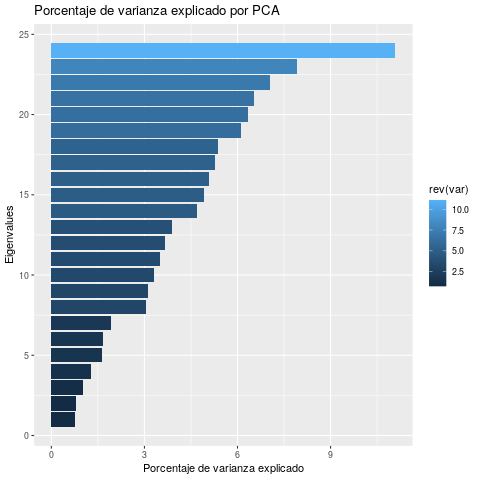
\includegraphics[width=0.4\textwidth]{PCA_var.png}
    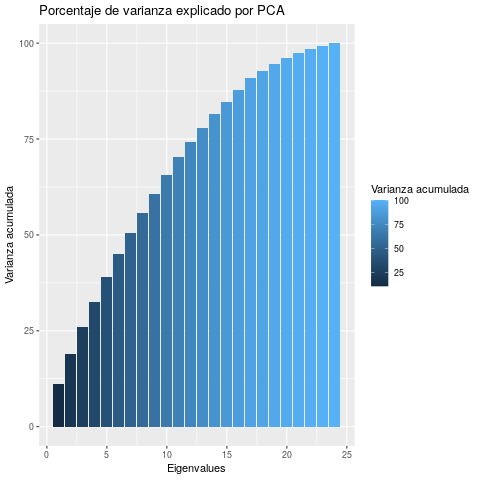
\includegraphics[width=0.4\textwidth]{PCA_var_acumulada.png}
    \caption{Porcentaje explicado de varianza. Varianza acumulada}
    \label{fig:PCA_var}
\end{figure}


Se presenta la comparación de los análisis PCA y DAPC. Se observa claramente como el PCA no puede clasificar las poblaciones debido a su estructura pero el DA sí lo logra hacer. 


\begin{figure}[h]
    \centering
    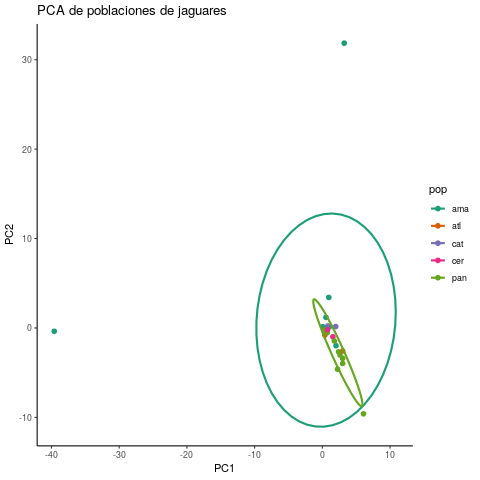
\includegraphics[width=0.4\textwidth]{PCA_plot.png}
    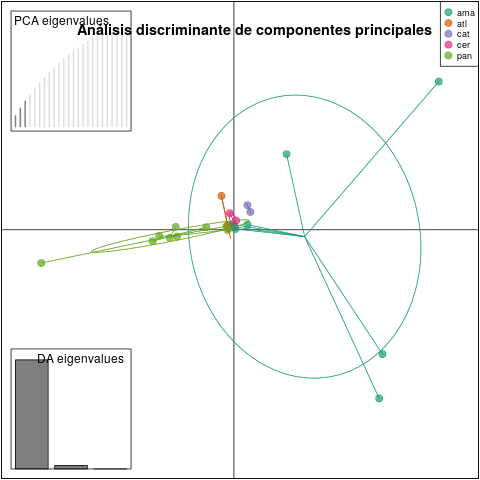
\includegraphics[width=0.4\textwidth]{DAPC.png}
    \caption{Panel izquierdo, PCA de poblaciones de jaguares. Panel derecho Análisis discriminante de componentes principales}
    \label{fig:PCA_DA}
\end{figure}



\begin{figure}[ht]
    \centering
    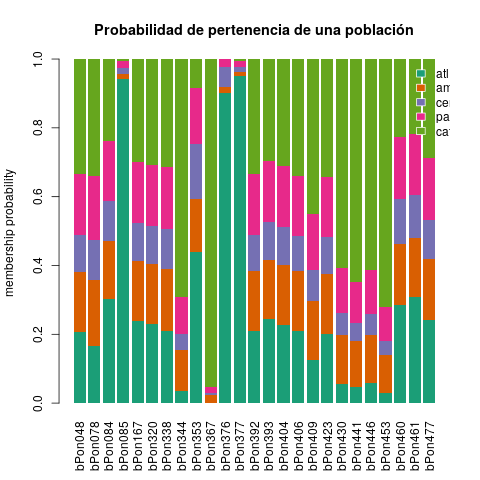
\includegraphics[width=0.4\textwidth]{compoplot.png}
    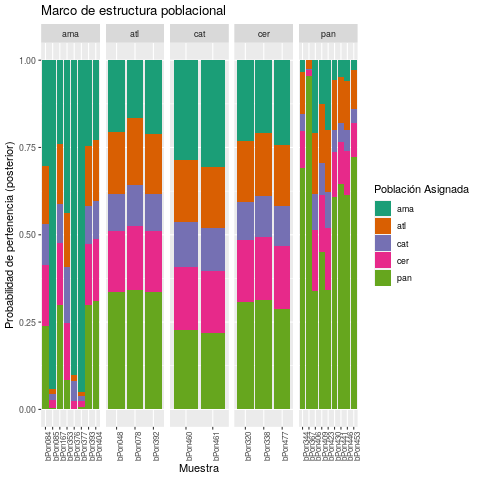
\includegraphics[width=0.4\textwidth]{estructura_poblacional.png}
    \caption{Panel izquierdo: probabilidad de pertenencia para una población para cada muestra. Panel derecho: Población asignada para cada muestra}
    \label{fig:estructura}
\end{figure}

Finalmente se calcula la probabilidad de pertenencia de una población. Como una consecuencia del análisis discriminante (DA) se genera una probabilidad de pertenencia dado un grupo \textit{a priori}, logrando clasificar las muestras en diferentes poblaciones dada su información.

\newpage

\subsection{Código en R}
A continuación se presenta el código utilizado para generar los análisis en R

\begin{lstlisting}[language=R]

list.of.packages <- c("vcfR",
                      "poppr",
                      "ape",
                      "RColorBrewer",
                      "dplyr",
                      "tidyverse",
                      "adegenet",
                      "igraph")
new.packages <- list.of.packages[!(list.of.packages %in% installed.packages()[,"Package"])]
if(length(new.packages)) install.packages(new.packages, repos = "https://cloud.r-project.org/")
sapply(list.of.packages, require, character.only = TRUE)

dir.create("data")

#Abrir el archivo VCF usando vcfR y verificar que esten las muestras y SNPs cargados.
jaguar.VCF <- read.vcfR("data/populations.snps.vcf")


#Cargar la información sobre la población en un archivo .txt.Este incluye ID y nombre de la población.
#Usar la función read.table():
pop.data <- read.table("data/pop_map_25smp.txt", sep = "\t", header = FALSE, col.names = c("AccesID", "population")) 

pop_data <- readr::read_tsv("data/pop_map_25smp.txt", col_names =  FALSE) %>% 
  dplyr::rename(AccesID = X1) %>% 
  dplyr::rename(population = X2)
populations <- distinct(pop_data, population) %>% pull()
jaguar_vcf <- jaguar.VCF@gt %>% tibble::as_tibble() 

jaguar_vcf_gather <- jaguar_vcf %>% 
  tidyr::gather(AccesID, Info, -FORMAT) %>% 
  na.exclude() 

#Verificar que todas las muestras en el VCF y la tabla de datos de población estén incluidas.
val <- dplyr::distinct(jaguar_vcf_gather, AccesID) %>% 
    dplyr::anti_join(pop.data_tibble) %>%
  nrow 
ifelse(val != 0, "some populations are missing!", "All populations in VFC ok" )




#Convertir el objeto vcfR en un objeto genlight, usando la función: vcfR2genlight:
gl.jaguar <- vcfR::vcfR2genlight(jaguar.VCF)

#Especificar la ploidía del organismo
ploidy(gl.jaguar) <- 2

#Agregar la información sobre las poblaciones al objeto genlight
pop(gl.jaguar) <- pop_data$population

#Crear una matriz de distancia genética a partir de objetos genlight, con la función bitwise.dist().

geneticDistance <- poppr::bitwise.dist(gl.jaguar,
                              percent = TRUE,
                              mat = FALSE,
                              missing_match = TRUE,
                              scale_missing = FALSE,
                              euclidean = FALSE,
                              differences_only = FALSE,
                              threads = 3L
)



png("data/heatmap_distance.png", 640, 640)
heatmap(as.matrix(geneticDistance))
legend(x="bottomright", legend=c("min", "ave", "max"), 
       fill=colorRampPalette(brewer.pal(8, "Oranges"))(3))
title("Mapa de calor entre las distancias bit a bit de todas las muestras")
dev.off()
geneticDistanceTibble <- geneticDistance %>% 
  broom::tidy() %>% 
  rename(population_1 = item1, population_2 = item2)
library(igraph)

png("data/boxplot_distancia.png", 480, 480)

geneticDistanceTibble %>% 
  ggplot(aes(population_1, distance)) + geom_boxplot() + 
  coord_flip() + 
  xlab("Población 1") + 
  ylab("Distancia genética (proporción de loci diferentes") + 
  ggtitle("Distancia genética de una población con respecto a las demás")
dev.off()
#Construir un árbol de distancia genética para representar la relación genética de las muestras. 

tree <- poppr::aboot(gl.jaguar, tree = "upgma", distance = bitwise.dist, sample = 100, showtree = FALSE, cutoff = 50, quiet = T)
cols <- brewer.pal(n = length(populations), name = "Dark2")
?aboot
library(ggtree)
#Representación gráfica del árbol 

png("data/arbol_jaguar.png", 480, 480)
plot(tree, cex = 0.8, font = 2, adj = 0, tip.color =  cols[pop(gl.jaguar)], type = "phylogram")
legend('topleft',
       legend = populations,
       fill = cols, border = FALSE, bty = "n", cex = 1)
axis(side = 1)
title(xlab = "Distancia genética (proporción de loci diferentes)")
dev.off()

#Construcción de redes de expasión mínima, a través del objeto genlight objeto y una matriz de distancia.
jaguar.dist <- poppr::bitwise.dist(gl.jaguar)
jaguar.msn <- poppr::poppr.msn(gl.jaguar, jaguar.dist, showplot = TRUE, include.ties = T)
?poppr::poppr.msn

#Representación gráfica de la red.
node.size <- rep(2, times = nInd(gl.jaguar))
names(node.size) <- indNames(gl.jaguar)
vertex.attributes(jaguar.msn$graph)$size <- node.size
#set.seed(1)

png("data/grafo_red_jaguar.png", 480, 480)
plot_poppr_msn(gl.jaguar, jaguar.msn ,
               palette =  cols, gadj = 70)

dev.off()

?plot_poppr_msn
#Realizar un PCA con el objeto genlight usando la función  glPCA.
jaguar.pca <- adegenet::glPca(gl.jaguar, nf = 3)

png("data/PCA_var.png", 480, 480)

tibble(var = 100 * jaguar.pca$eig/sum(jaguar.pca$eig) ) %>% 
  mutate(PCA = row_number()) %>% 
  ggplot() + 
  geom_bar(aes(PCA, rev(var), fill = rev(var)), stat = "identity") + 
  coord_flip() + 
  ggtitle("Porcentaje de varianza explicado por PCA") + 
  xlab("Eigenvalues") + 
  ylab("Porcentaje de varianza explicado")

dev.off()



png("data/PCA_var_acumulada.png", 480, 480)

tibble(var = 100 * jaguar.pca$eig/sum(jaguar.pca$eig) ) %>%
  mutate(var_acummulated = cumsum(var)) %>% 
  mutate(PCA = row_number()) %>% 
  ggplot() + 
  geom_bar(aes(PCA, (var_acummulated), fill = (var_acummulated)), stat = "identity") + 
  #coord_flip() + 
  ggtitle("Porcentaje de varianza explicado por PCA") + 
  xlab("Eigenvalues") + 
  ylab("Varianza acumulada") + 
  scale_fill_continuous(name = "Varianza acumulada")

dev.off()
barplot( 100 * jaguar.pca$eig/sum(jaguar.pca$eig),
         col = heat.colors(50), 
         main="PCA Eigenvalues")
title(ylab="Percent of variance\nexplained", line = 2)
title(xlab="Eigenvalues", line = 1)

#Ver los resultados de PCA
jaguar.pca.scores <- as_tibble(jaguar.pca$scores) %>% 
  mutate(pop = pop(gl.jaguar)) 
library(ggplot)

p <- jaguar.pca.scores %>% 
  ggplot(aes(x=PC1, y=PC2, col = pop)) +
  geom_point(size=2) +
  stat_ellipse(level = 0.95, size = 1) +
  scale_color_manual(values = cols) +
  #geom_hline(yintercept = 0) +
  #geom_vline(xintercept = 0) +
  theme_classic() + 
  ggtitle("PCA de poblaciones de jaguares")

png("data/PCA_plot.png", 480, 480)
p
dev.off()
#Análisis discriminante de componentes principales (DAPC), para maximizar la varianza entre poblaciones.

pnw.dapc <- dapc(gl.jaguar, n.pca = 3, n.da = 2)


#Para confirmar que el DAPC es similar al PCA, trazar los datos en un diagrama de dispersión.

png("data/DAPC.png", 480, 480)
ade4::scatter(pnw.dapc, col = cols, cex = 2, legend = TRUE, clabel = F, posi.leg = "topright", scree.pca = TRUE,
        posi.pca = "topleft", cleg = 0.75, posi.da = "bottomleft" )
title("Análisis discriminante de componentes principales")
dev.off()
#Visualizar las asignaciones posteriores de cada muestra a una población, a traves del diagrama compuesto de barras apiladas.

png("data/compoplot.png", 480, 480)
adegenet::compoplot(pnw.dapc, col = cols, posi = NA, show.lab = TRUE, )
legend("topright",
       inset=c(-0.04,0),
       legend = populations,
       fill = cols, border = FALSE, bty = "n", cex = 1)
title("Probabilidad de pertenencia de una población")

dev.off()

#Separar las muestras por población.
#Observación de probabilidad de pertenencia para una población: nombre de la muestra, la población original y la población asignada


dapc_results <- pnw.dapc$posterior %>% 
  as_tibble() %>% 
  mutate(pop = pop(gl.jaguar)) %>% 
  mutate(Sample = rownames(pnw.dapc$posterior)) %>% 
  tidyr::gather(Assigned_Pop, Posterior_membership_probability, -pop, -Sample) %>% 
  rename(Original_Pop = pop) 
  

#Rpresentación gráfica del marco de estructura poblacional
png("data/estructura_poblacional.png", 480, 480)
dapc_results %>% 
  ggplot(aes(x=Sample, y=Posterior_membership_probability, fill=Assigned_Pop)) +
  geom_bar(stat = 'identity') +
  scale_fill_manual(values = cols, name = "Población Asignada") +
  facet_grid(~Original_Pop, scales = "free") +
  theme(axis.text.x = element_text(angle = 90, hjust = 1, size = 8)) + 
  ylab("Probabilidad de pertenencia (posterior)") +
  xlab("Muestra") + 
  #coord_flip() +
  ggtitle("Marco de estructura poblacional")
dev.off()
\end{lstlisting}


\bibliography{library}
\end{document}
